%%%%%%%%%%%%%%%%%%%%%%%%%%%%%%%%%%%%%%%%%
% Title
% Project No. 
%
% Author: bmarron
% Origin: 
% Final:
%
% INSERT doc content into "ARTICLE CONTENTS" 
% MODIFY the "TITLE SECTION"
% MODIFY path references for all figures
%%%%%%%%%%%%%%%%%%%%%%%%%%%%%%%%%%%%%%%%%



%----------------------------------------------------------------------------------------
%	PACKAGES AND OTHER DOCUMENT CONFIGURATIONS
%----------------------------------------------------------------------------------------

\documentclass[twoside]{article}	%use

\usepackage{lipsum} % Package to generate dummy text throughout this template
\usepackage{csquotes}
\usepackage[natbibapa]{apacite}
\usepackage[english]{babel}
\usepackage{amsmath}
\usepackage{amsthm}
\usepackage{amssymb}
\usepackage{pdfpages}
\usepackage{verbatim}
\usepackage{bigfoot}
\usepackage{multirow}


\usepackage[sc]{mathpazo} % Use the Palatino font and the Pazo fonts for math
\usepackage[T1]{fontenc} % Use 8-bit encoding that has 256 glyphs
\linespread{1.05} % Line spacing - Palatino needs more space between lines
\usepackage{microtype} % Slightly tweak font spacing for aesthetics

\usepackage[hmarginratio=1:1,top=32mm,columnsep=20pt]{geometry} % Document margins
\usepackage{multicol} % Used for the two-column layout of the document
\usepackage[hang, small,labelfont=bf,up,textfont=it,up]{caption} % Custom captions under/above floats in tables or figures
\usepackage{booktabs} % Horizontal rules in tables
\usepackage{float} % Required for tables and figures in the multi-column environment - they need to be placed in specific locations with the [H] (e.g. \begin{table}[H])
%\usepackage{hyperref} % Interferes with cite.sty 

%\usepackage{lettrine} % The lettrine is the first enlarged letter at the beginning of the text
\usepackage{paralist} % Used for the compactitem environment which makes bullet points with less space between them

\usepackage{abstract} % Allows abstract customization
\renewcommand{\abstractnamefont}{\normalfont\bfseries} % Set the "Abstract" text to bold
\renewcommand{\abstracttextfont}{\normalfont\small\itshape} % Set the abstract itself to small italic text

\usepackage{titlesec} % Allows customization of titles
\renewcommand\thesection{\Roman{section}} % Roman numerals for the sections
\renewcommand\thesubsection{\arabic{subsection}} % Arabic numerals for subsections
\titleformat{\section}[block]{\large\scshape\centering}{\thesection.}{1em}{} % Change the look of the section titles
\titleformat{\subsection}[block]{\large}{\thesubsection.}{1em}{} % Change the look of the section titles

\usepackage{fancyhdr} % Headers and footers
\pagestyle{fancy} % All pages have headers and footers
\fancyhead{} % Blank out the default header
\fancyfoot{} % Blank out the default footer
\fancyhead[R]{\date{\today}}
\fancyfoot[R]{\thepage} % Custom footer text
%\fancyhead[C]{Running title $\bullet$ November 2012 $\bullet$ Vol. XXI, No. 1} % Custom header text
%\fancyfoot[RO,LE]{\thepage} % Custom footer text

%-------------------------------------------------------------
% NEW COMMANDS
%---------------------------------------------------------------------
%This command creates a box marked ``To Do'' around text.
%To use type \todo{  insert text here  }.
\newcommand{\todo}[1]{\vspace{5 mm}\par \noindent
\marginpar{\textsc{To Do}}
\framebox{\begin{minipage}[c]{0.95 \textwidth}
\tt\begin{center} #1 \end{center}\end{minipage}}\vspace{5 mm}\par}


\newcommand{\sun}{\ensuremath{\odot}} % sun symbol is \sun


% To use paragraph indents
%\begin{myindentpar}{2em}
% blah blah blah
%\end {myindentpar}
\newenvironment{myindentpar}[1]%
   {\begin{list}{}%
       {\setlength{\leftmargin}{#1}}%
           \item[]%
   }
     {\end{list}}

%----------------------------------------------------------------------------------------
%	TITLE SECTION
%----------------------------------------------------------------------------------------

\title{\vspace{-15mm}\fontsize{14pt}{10pt}\selectfont\textbf{QAQC Updates}} % Article title

\author{
\large
\textsc{Bruce D. Marron} \\ %\thanks{A thank you or further information}\\[2mm] % Your name
\normalsize LANDIS-II Upgrades Project \\ % Your institution
\vspace{-5mm}
}
\date{}

%----------------------------------------------------------------------------------------
\begin{document}
\maketitle                % Insert title
\thispagestyle{fancy}     % All pages have headers and footers

%----------------------------------------------------------------------------------------
%	ABSTRACT
%----------------------------------------------------------------------------------------

%\begin{abstract}

%end{abstract}

%----------------------------------------------------------------------------------------
%	ARTICLE CONTENTS
%----------------------------------------------------------------------------------------

\section{OpenIssues}
\footnotesize 
\verbatiminput{/home/bmarron/Desktop/PSU/PhD_EES/2016SoE021_LANDIS_Upgrades_Project/Works_InProgress/OpenIssues_GitHub.txt}

\section{Salvage Logging}
\verbatiminput{/home/bmarron/Desktop/PSU/PhD_EES/2016SoE021_LANDIS_Upgrades_Project/Works_InProgress/ProjectWorkLogs/PWL50_QAQC-SalvageLogBiomassHrvst_20170226.txt}

\begin{figure} [!htbp]
  \begin{center}
    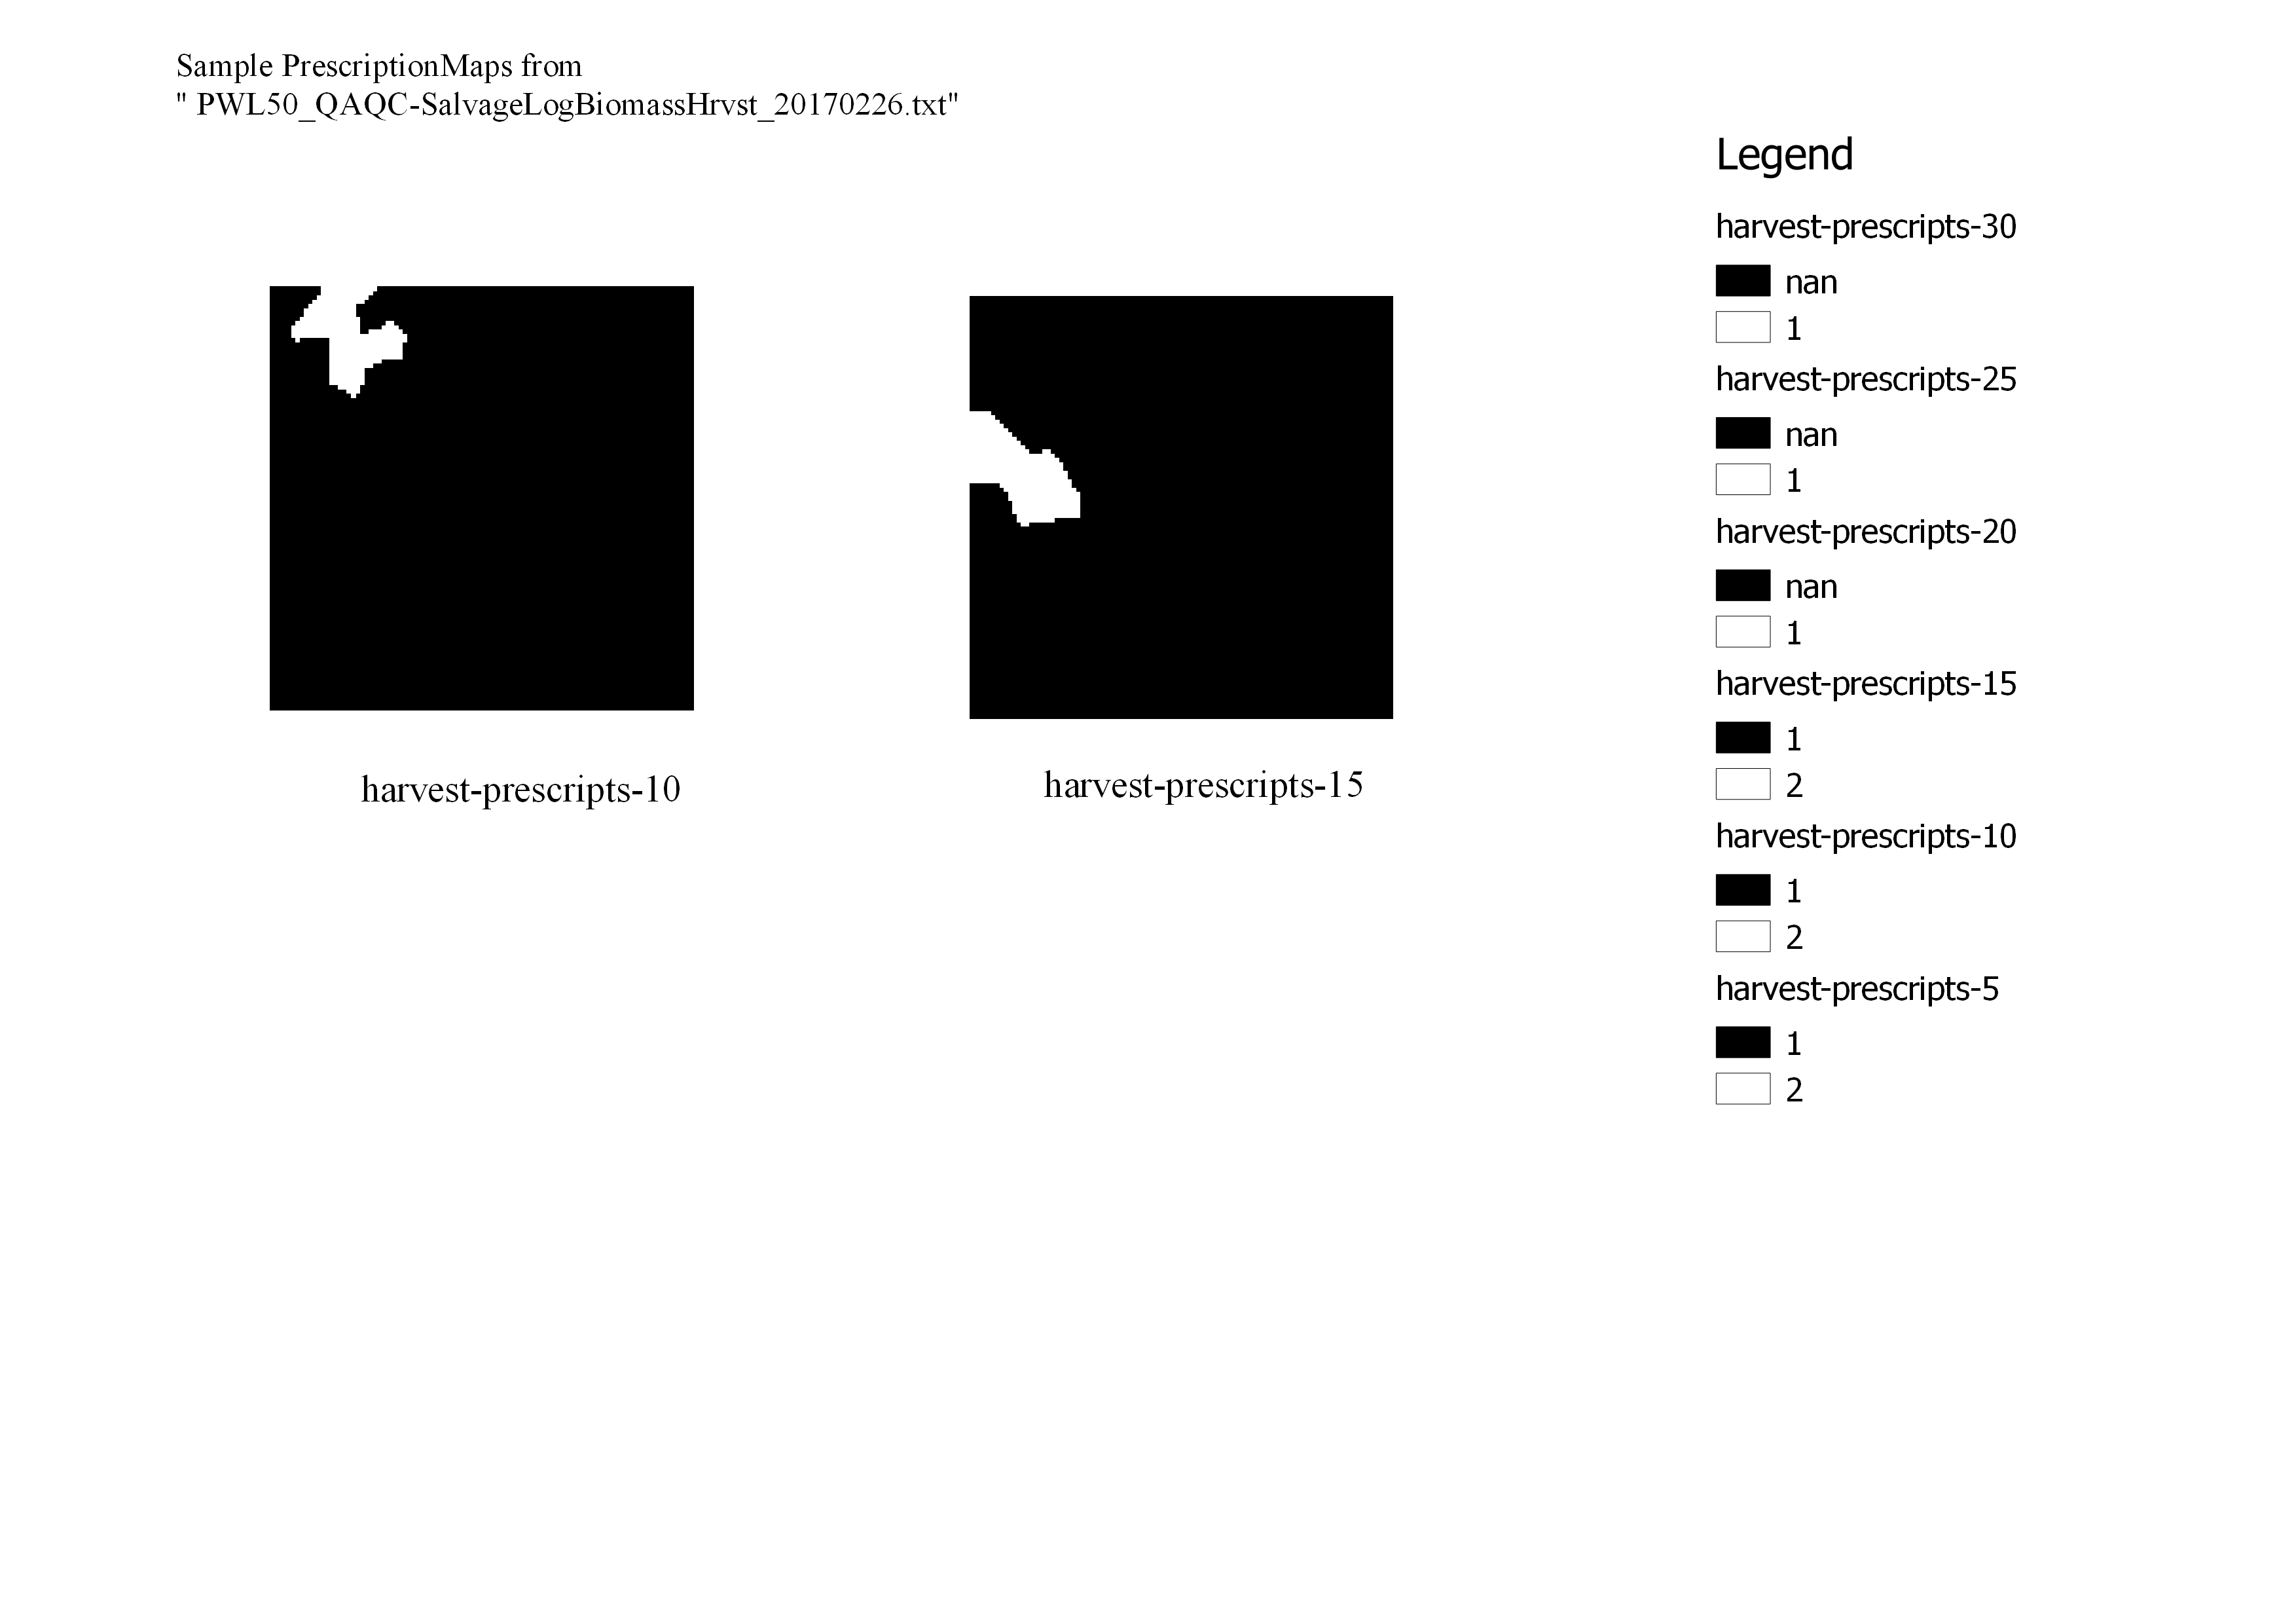
\includegraphics[scale = 0.6]{graphics/PWL50_PrescriptionMaps_QAQCrun1}
    \caption{}
    \label{fig:}
  \end{center}
\end{figure}

\begin{figure}[!htbp]
  \begin{center}
    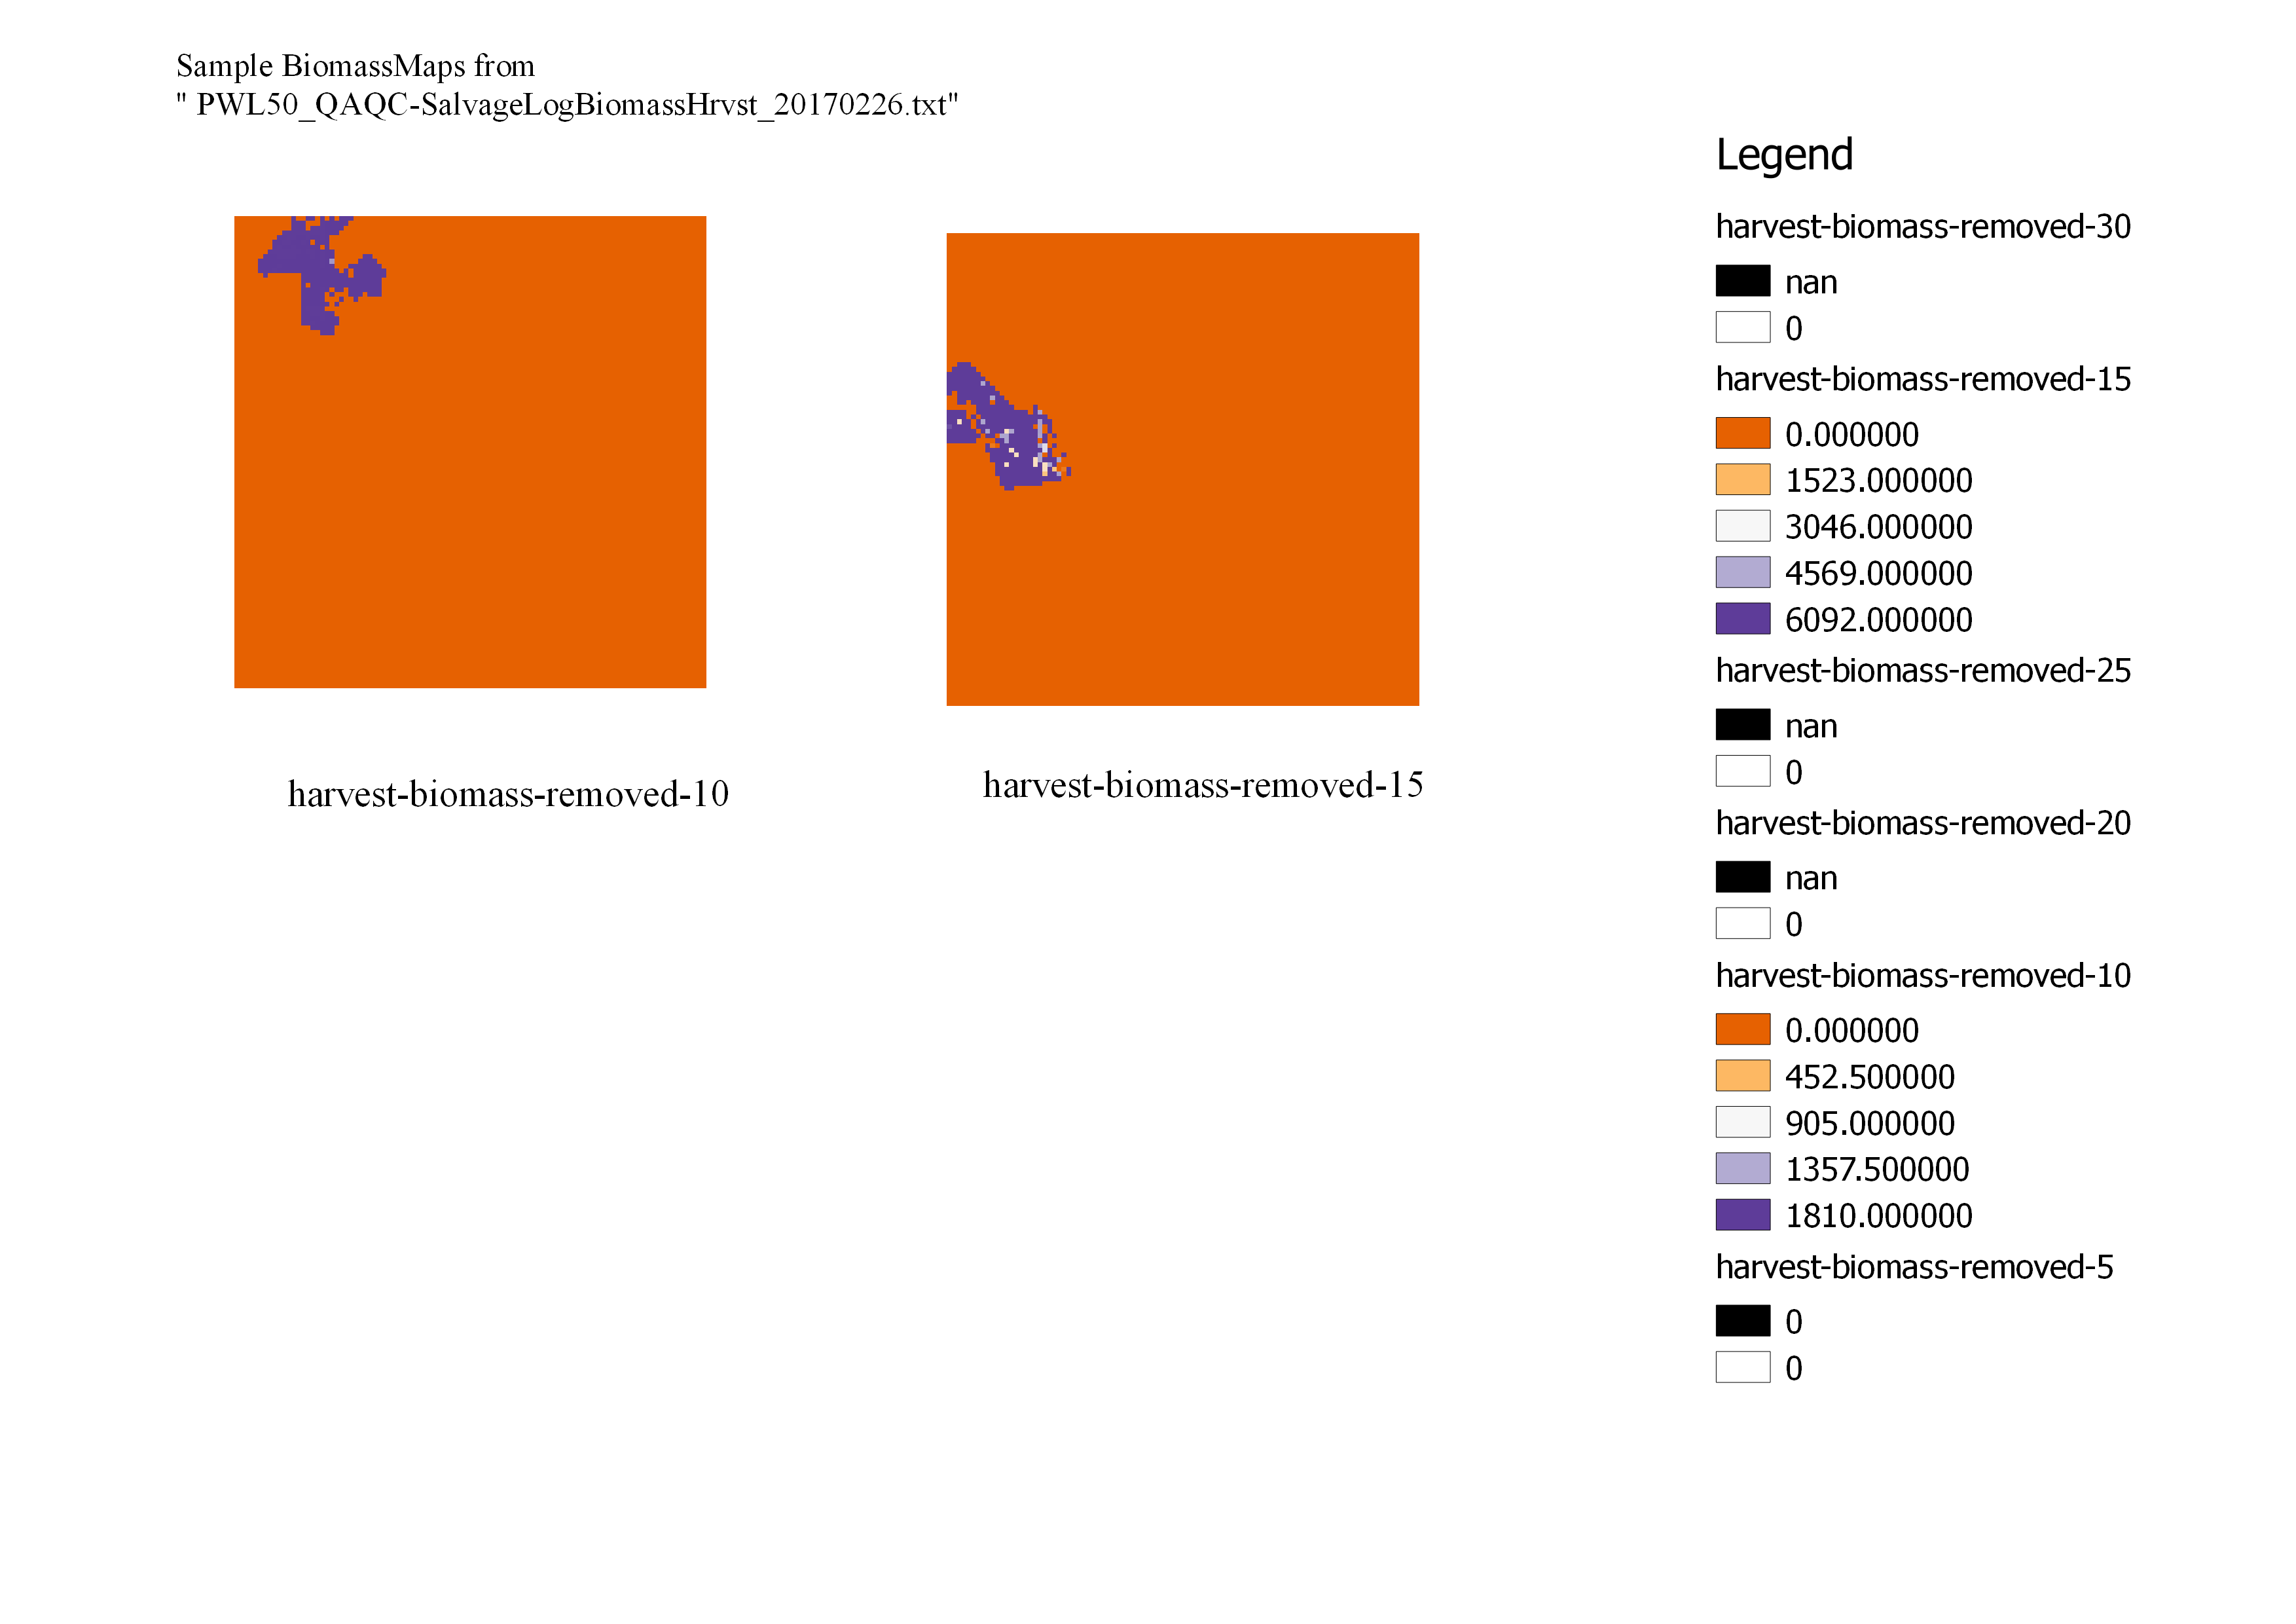
\includegraphics[scale = 0.6]{graphics/PWL50_BiomassMaps_QAQCrun1}
    \caption{}
    \label{fig:}
  \end{center}
\end{figure}

\begin{figure}[!htbp]
  \begin{center}
    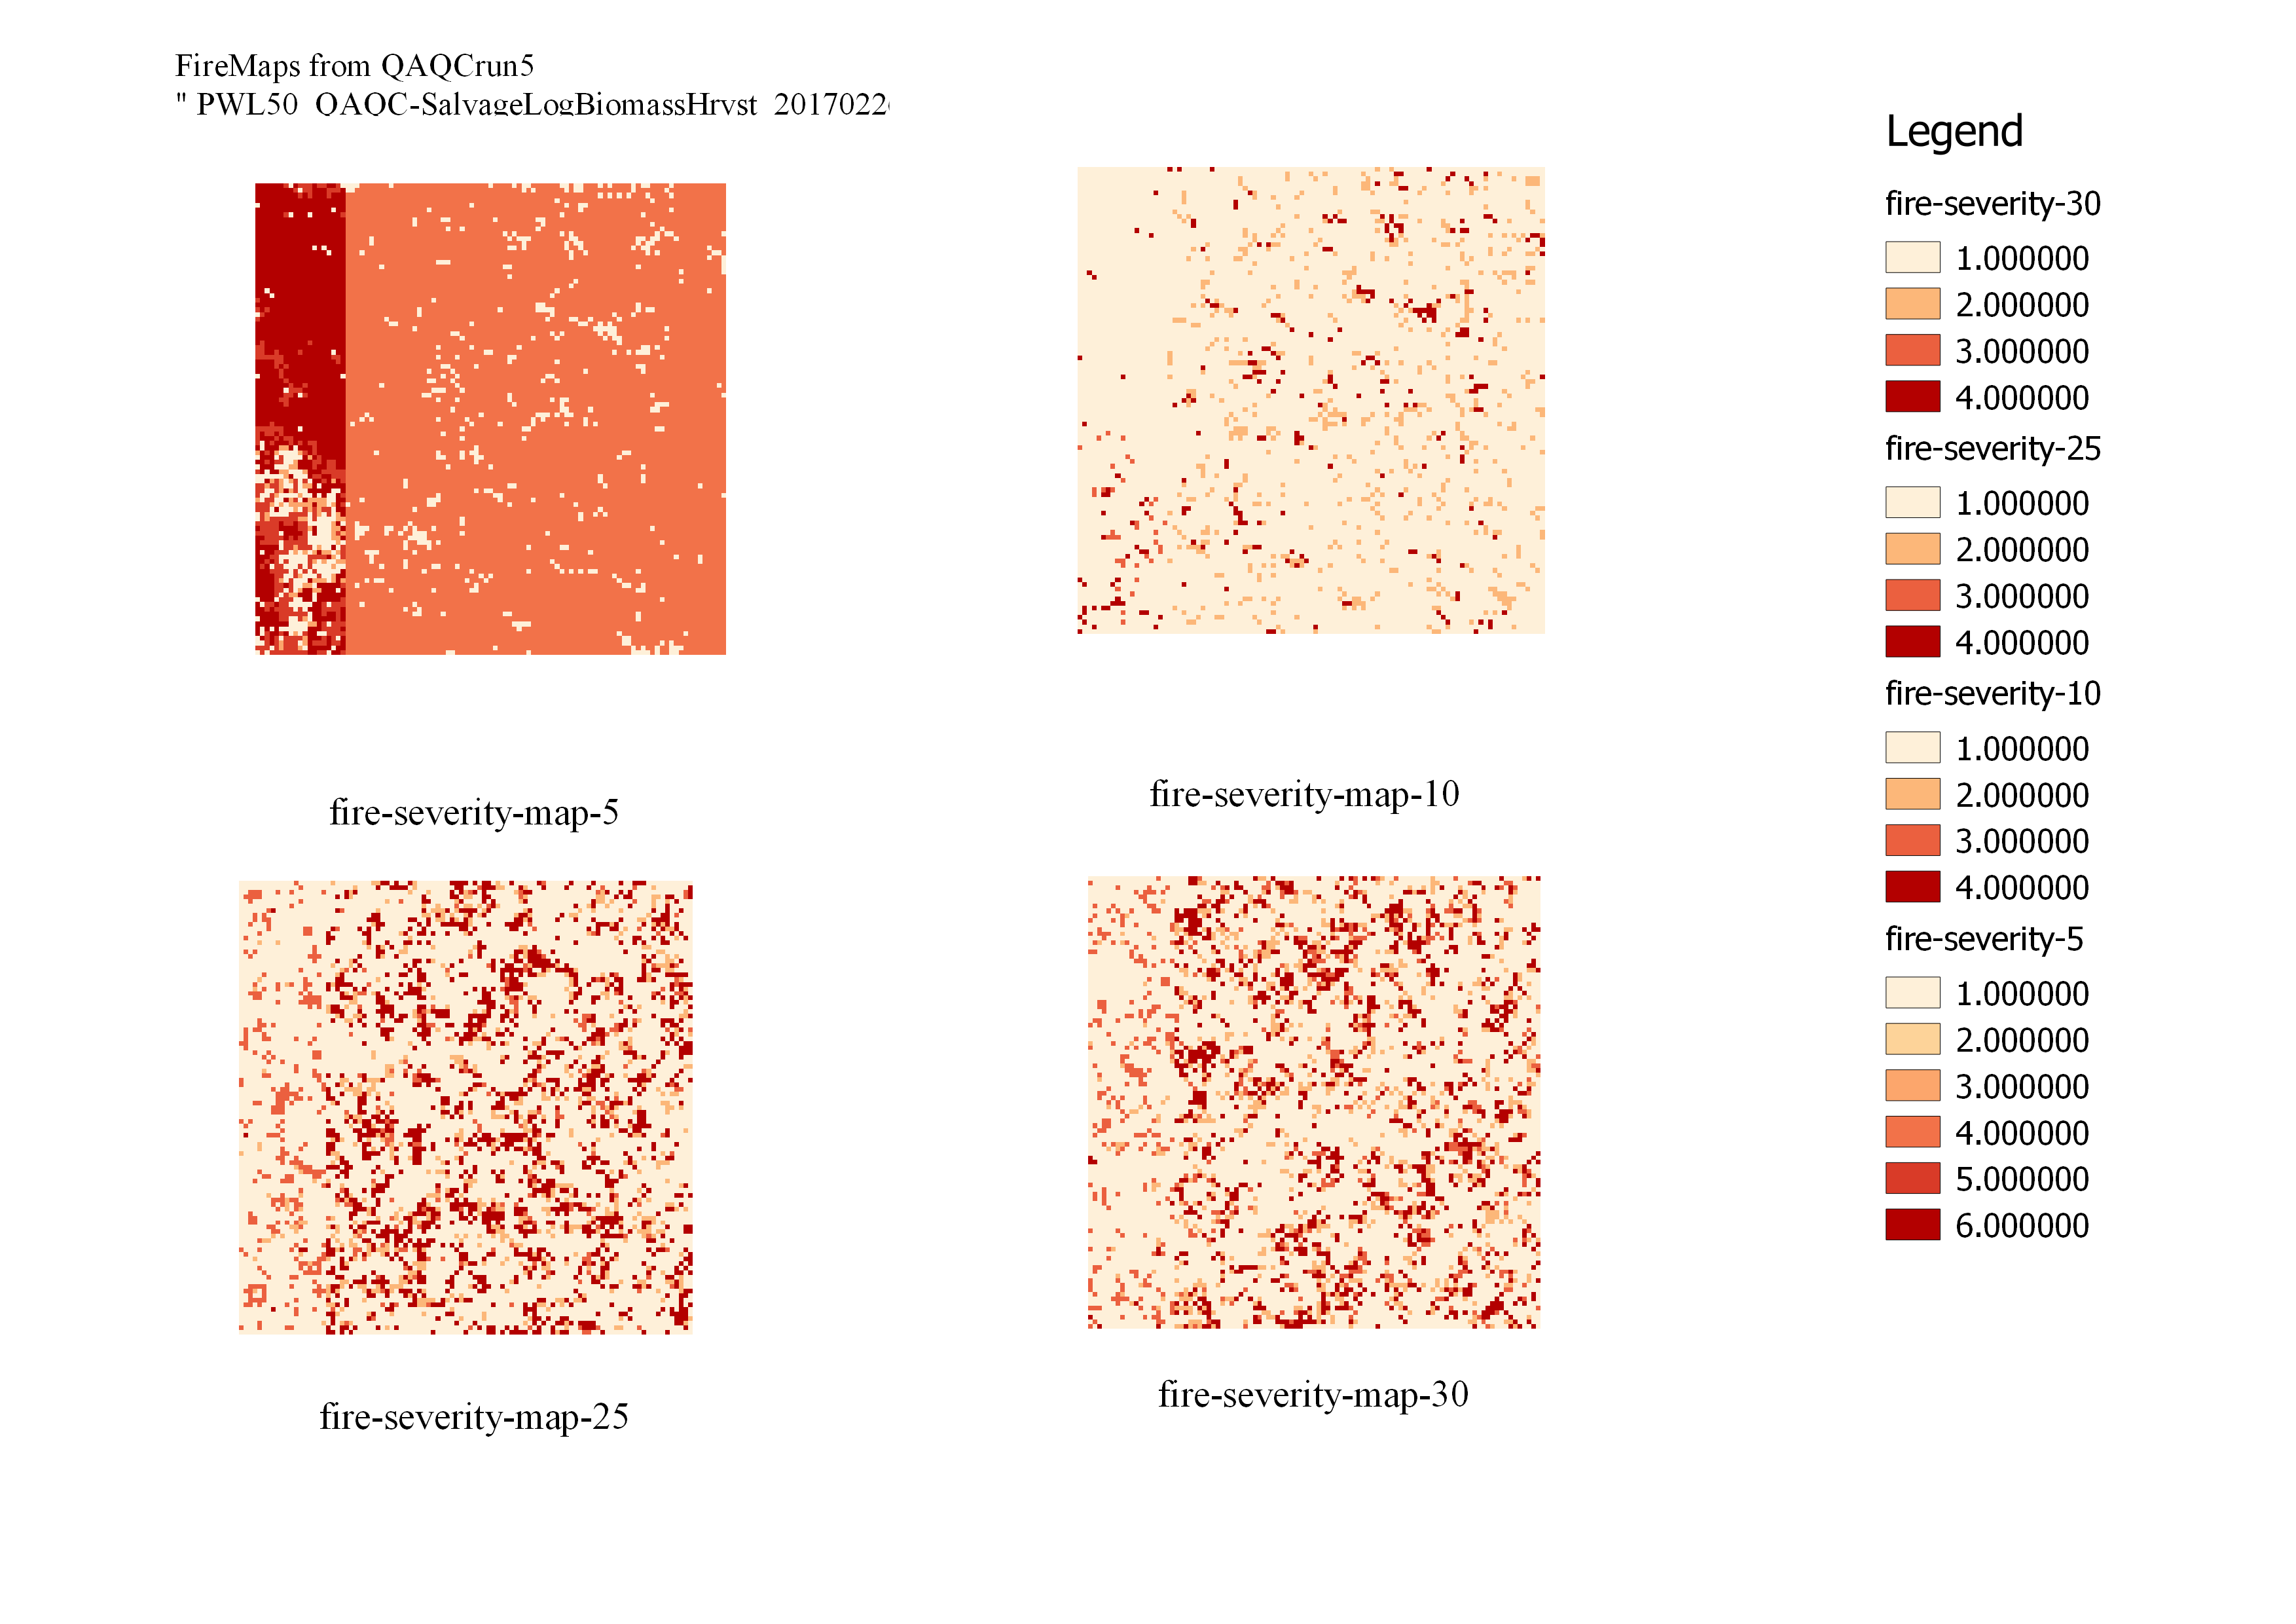
\includegraphics[scale = 0.6]{graphics/PWL50_FireMaps_QAQCrun5}
    \caption{}
    \label{fig:}
  \end{center}
\end{figure}


%----------------------------------------------------------------------------------------
%	REFERENCE LIST
%----------------------------------------------------------------------------------------
\newpage
\bibliographystyle{/usr/local/share/texmf/tex/latex/apacite/apacite}
\bibliography{/home/bmarron/Desktop/BibTex/My_Library_20170125}


\end{document}
